\documentclass{article}%
\usepackage[T1]{fontenc}%
\usepackage[utf8]{inputenc}%
\usepackage{lmodern}%
\usepackage{textcomp}%
\usepackage{lastpage}%
\usepackage{geometry}%
\geometry{tmargin=2cm,lmargin=2cm,rmargin=2cm,bmargin=2cm}%
\usepackage{graphicx}%
\usepackage{float}%
\usepackage{booktabs}%
%
\title{Relatório de Análise de Performance dos Modelos de Resposta}%
\date{\today}%
%
\begin{document}%
\normalsize%
\maketitle%
\section*{Introdução}%
\label{sec:Introduo}%
Este relatório apresenta uma análise completa dos modelos de resposta, avaliando a similaridade entre as respostas geradas e as respostas de referência. Foram calculadas diversas métricas de similaridade e realizadas análises estatísticas e visuais para identificar padrões de performance, inconsistências e possíveis pontos de melhoria. O objetivo é fornecer subsídios para interpretar os dados de forma objetiva, auxiliando na tomada de decisões para ajustes nos algoritmos.

%
\section*{Metodologia}%
\label{sec:Metodologia}%
A análise foi realizada em duas etapas principais:\newline%
\newline%
%
\begin{itemize}%
\item Carregamento dos dados: os dados foram extraídos de um arquivo pickle e convertidos para dicionários, possibilitando o acesso às respostas dos modelos e às respostas de referência.%
\item Processamento e análise: foram calculadas diversas métricas de similaridade, estatísticas descritivas e correlações. Além disso, foram gerados diversos gráficos (barras, histogramas, boxplots, heatmaps e scatter plots) para facilitar a interpretação visual dos resultados.%
\end{itemize}%
Cada gráfico ou tabela vem acompanhado de uma breve explicação sobre como interpretá{-}lo, de modo que o leitor possa compreender os pontos principais de cada análise.

%
\section*{Resultados}%
\label{sec:Resultados}%
\subsection*{Estatísticas de Similaridade Geral}%
\label{subsec:EstatsticasdeSimilaridadeGeral}%
Nesta seção são apresentadas as estatísticas descritivas da overall similarity dos modelos. Valores médios e medianos mais elevados indicam melhor aderência às respostas de referência, enquanto um alto desvio padrão pode indicar maior variabilidade.%
\newline%
Foram gerados os seguintes gráficos para visualizar esses dados:%


\begin{figure}[H]%
\centering%
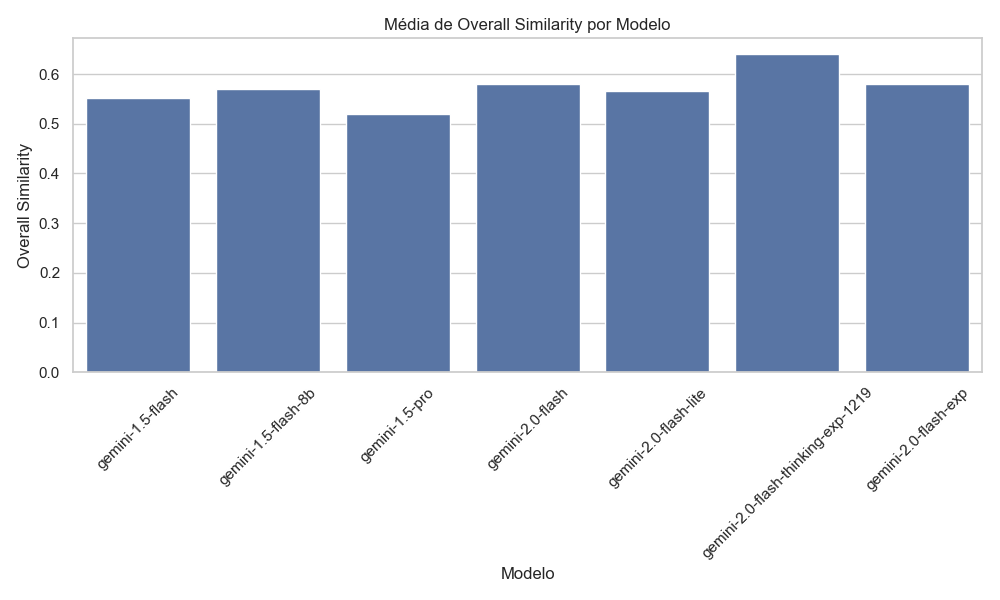
\includegraphics[width=0.8\textwidth]{analysis_results/barplot_overall_similarity.png}%
\caption{Gráfico de Barras – Média de Overall Similarity por Modelo. Observe as diferenças de desempenho entre os modelos.}%
\end{figure}

%


\begin{figure}[H]%
\centering%
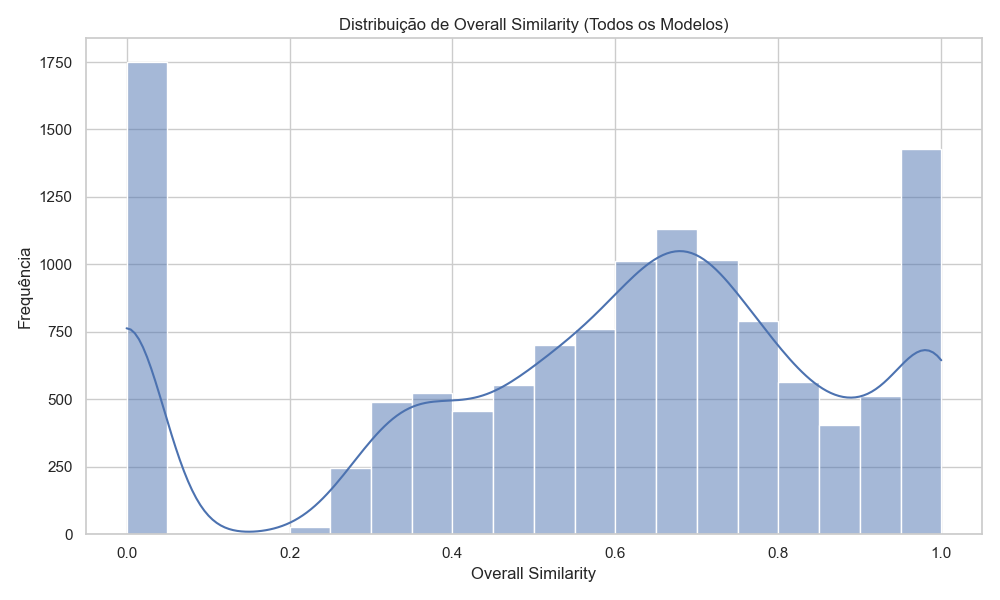
\includegraphics[width=0.8\textwidth]{analysis_results/histogram_overall_similarity.png}%
\caption{Histograma – Distribuição de Overall Similarity. Permite visualizar a dispersão dos valores obtidos.}%
\end{figure}

%


\begin{figure}[H]%
\centering%
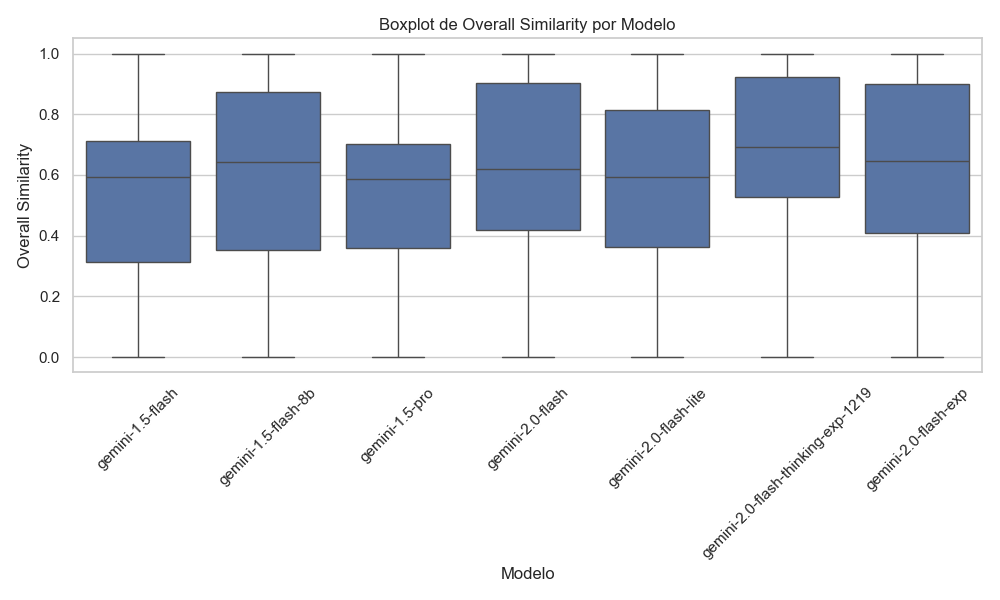
\includegraphics[width=0.8\textwidth]{analysis_results/boxplot_overall_similarity.png}%
\caption{Boxplot – Overall Similarity por Modelo. Facilita a identificação de mediana, quartis e outliers.}%
\end{figure}

%
\subsection*{Correlação entre Métricas de Similaridade}%
\label{subsec:CorrelaoentreMtricasdeSimilaridade}%
Nesta análise, avaliamos a correlação entre as diferentes métricas de similaridade (score keys). O heatmap abaixo mostra a força da correlação entre cada par de métricas: valores próximos de 1 ou {-}1 indicam forte correlação, enquanto valores próximos de 0 sugerem correlação fraca ou inexistente.%


\begin{figure}[H]%
\centering%
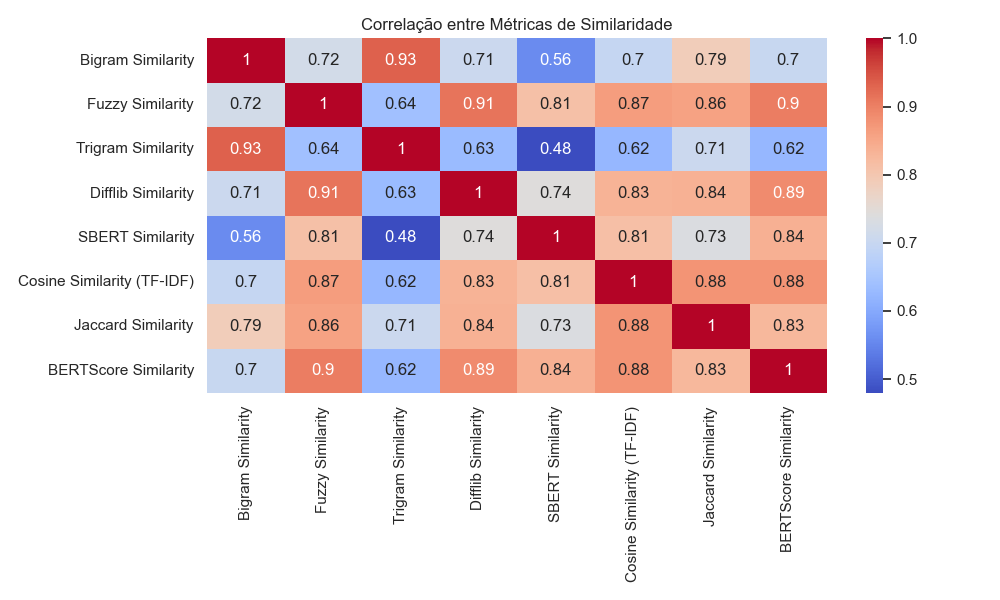
\includegraphics[width=0.8\textwidth]{analysis_results/heatmap_score_keys_correlation.png}%
\caption{Heatmap – Correlação entre as Métricas de Similaridade.}%
\end{figure}

%
\newline%
Além do heatmap, foram gerados scatter plots individuais comparando cada métrica com a overall similarity. Esses gráficos podem ser consultados nos anexos para análises mais detalhadas.

%
\subsection*{Correlação entre Overall Similarity e Média dos Scores}%
\label{subsec:CorrelaoentreOverallSimilarityeMdiadosScores}%
Esta seção apresenta a relação entre a overall similarity e a média dos scores detalhados (avg\textbackslash{}\_metric). O scatter plot a seguir permite identificar se existe uma tendência linear entre essas duas medidas, o que indicaria consistência na avaliação dos modelos.%


\begin{figure}[H]%
\centering%
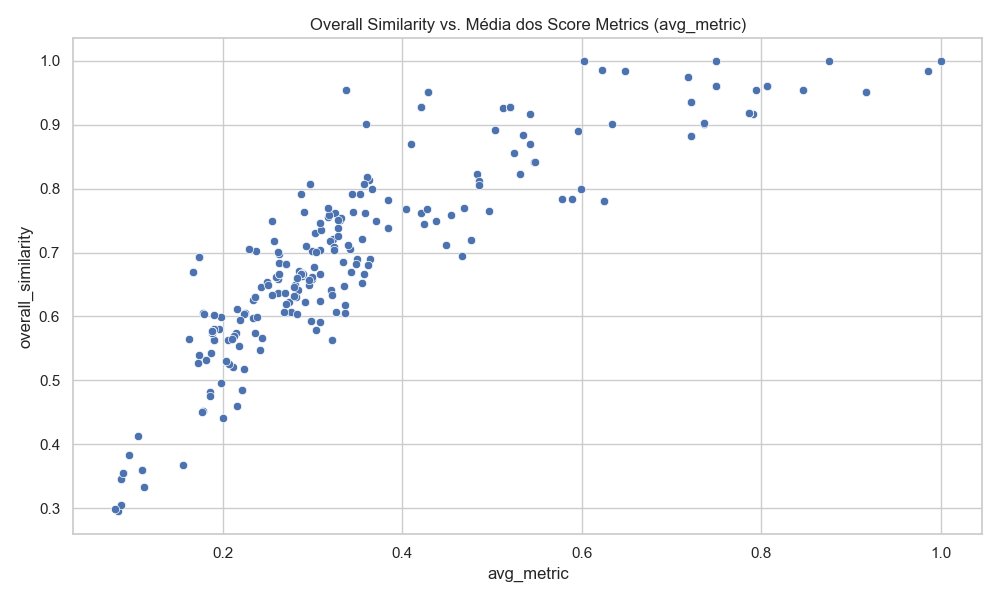
\includegraphics[width=0.8\textwidth]{analysis_results/scatter_overall_vs_avg_metric.png}%
\caption{Scatter Plot – Overall Similarity vs. Média dos Score Metrics (avg\textbackslash{}\_metric).}%
\end{figure}

%
\subsection*{Análise de Casos 'Unanswerable'}%
\label{subsec:AnlisedeCasosUnanswerable}%
Nesta parte, são analisados os casos em que os modelos não forneceram respostas (unanswerable). Os gráficos abaixo, apresentados lado a lado, mostram respectivamente a contagem desses casos e a relação entre a overall similarity e a condição de unanswerable. Em geral, uma baixa overall similarity pode estar associada a questões sem resposta.%


\begin{figure}[H]%
\begin{minipage}[b]{0.45\textwidth}%
\centering%
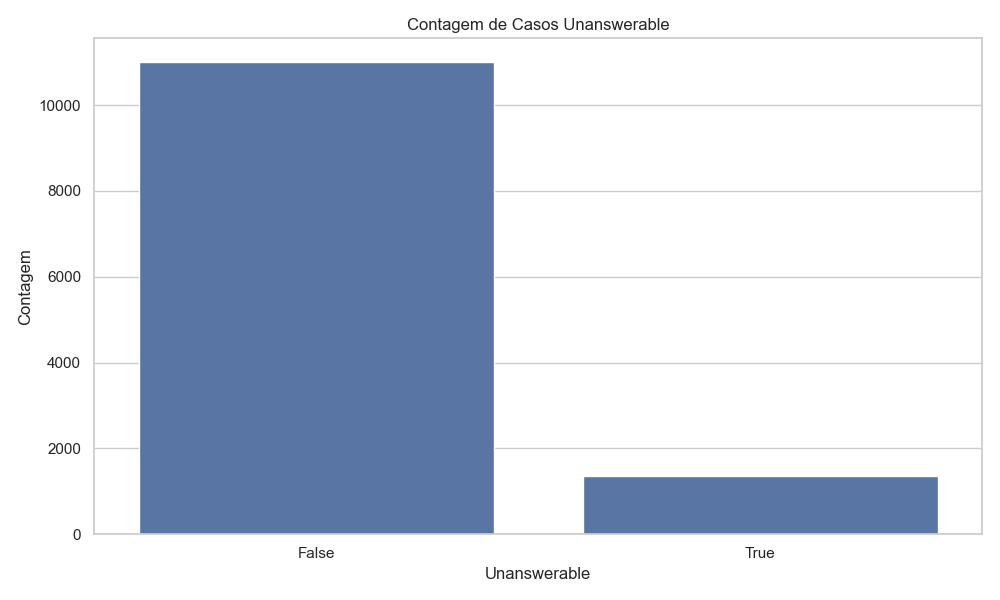
\includegraphics[width=\linewidth]{analysis_results\count_unanswerable.png}%
\caption*{Contagem de Casos Unanswerable.}%
\end{minipage}\hfill%
\begin{minipage}[b]{0.45\textwidth}%
\centering%
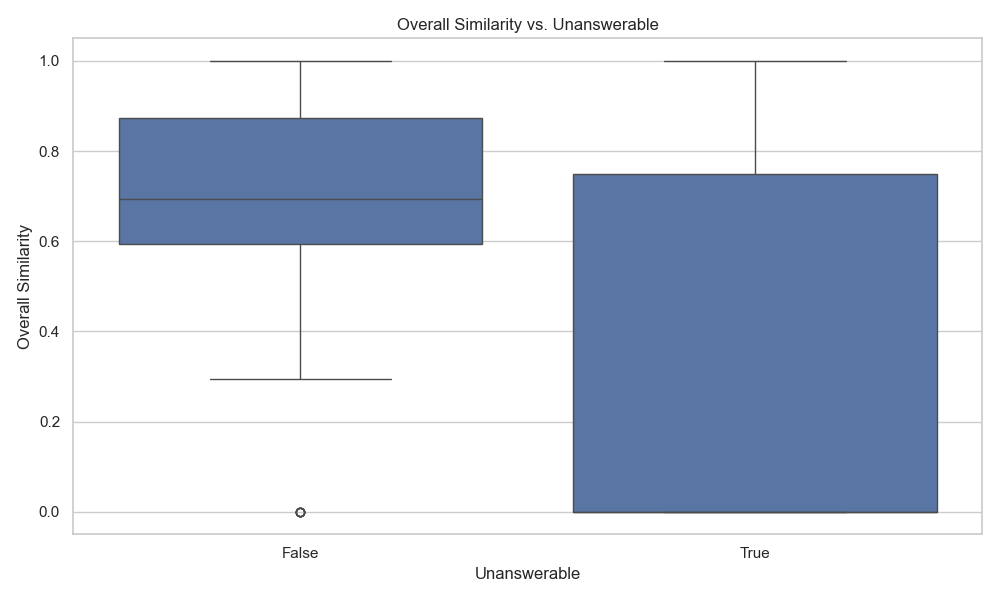
\includegraphics[width=\linewidth]{analysis_results\boxplot_overall_vs_unanswerable.png}%
\caption*{Boxplot – Overall Similarity vs. Unanswerable.}%
\end{minipage}%
\end{figure}

%
\subsection*{Correlação Inter{-}Modelos}%
\label{subsec:CorrelaoInter{-}Modelos}%
Esta análise verifica a correlação da overall similarity entre os diferentes modelos. Utilizando uma pivot table, foi calculada a correlação entre os modelos, cuja visualização por meio de um heatmap facilita a identificação de similaridades ou discrepâncias na performance entre eles.%


\begin{figure}[H]%
\centering%
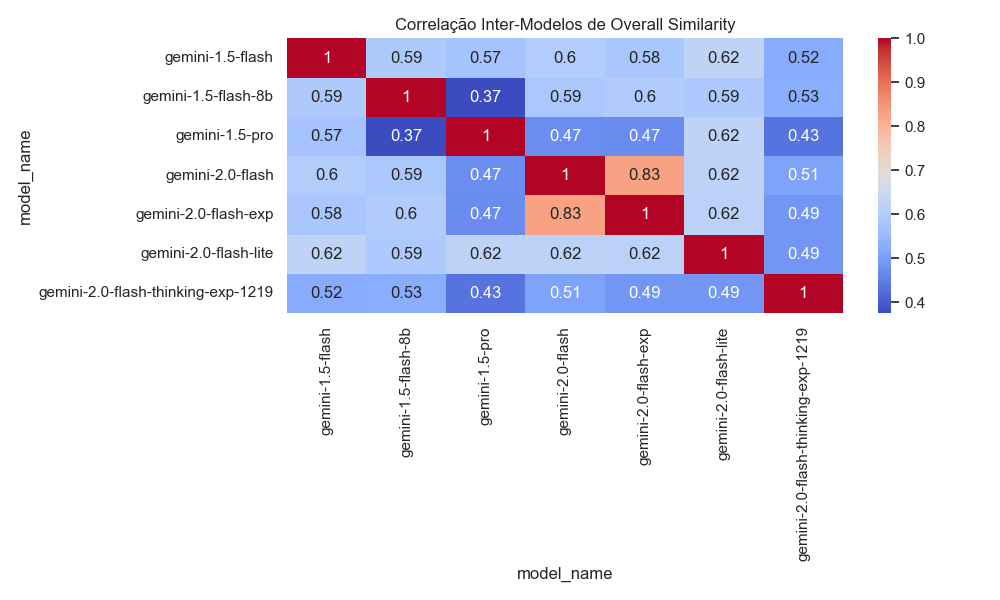
\includegraphics[width=0.8\textwidth]{analysis_results/heatmap_inter_model_corr.png}%
\caption{Heatmap – Correlação Inter{-}Modelos de Overall Similarity.}%
\end{figure}

%
\subsection*{Estatísticas Agregadas das Métricas Detalhadas}%
\label{subsec:EstatsticasAgregadasdasMtricasDetalhadas}%
Por fim, a tabela a seguir apresenta as estatísticas agregadas (média, mediana, desvio padrão, mínimo e máximo) para cada métrica detalhada, agrupadas por modelo. Essa análise auxilia na identificação de padrões e na avaliação da consistência dos scores.%
\begin{table}[H]%
\centering%
\caption{Estatísticas Agregadas das Métricas Detalhadas por Modelo}\label{tab:aggregated_metrics}%
\begin{tabular}{lllllllllllllllllllllllllllllllllllllllll}
\toprule
 & Difflib Similarity & Difflib Similarity.1 & Difflib Similarity.2 & Difflib Similarity.3 & Difflib Similarity.4 & Trigram Similarity & Trigram Similarity.1 & Trigram Similarity.2 & Trigram Similarity.3 & Trigram Similarity.4 & Jaccard Similarity & Jaccard Similarity.1 & Jaccard Similarity.2 & Jaccard Similarity.3 & Jaccard Similarity.4 & Fuzzy Similarity & Fuzzy Similarity.1 & Fuzzy Similarity.2 & Fuzzy Similarity.3 & Fuzzy Similarity.4 & SBERT Similarity & SBERT Similarity.1 & SBERT Similarity.2 & SBERT Similarity.3 & SBERT Similarity.4 & Bigram Similarity & Bigram Similarity.1 & Bigram Similarity.2 & Bigram Similarity.3 & Bigram Similarity.4 & BERTScore Similarity & BERTScore Similarity.1 & BERTScore Similarity.2 & BERTScore Similarity.3 & BERTScore Similarity.4 & Cosine Similarity (TF-IDF) & Cosine Similarity (TF-IDF).1 & Cosine Similarity (TF-IDF).2 & Cosine Similarity (TF-IDF).3 & Cosine Similarity (TF-IDF).4 \\
\midrule
NaN & mean & median & std & min & max & mean & median & std & min & max & mean & median & std & min & max & mean & median & std & min & max & mean & median & std & min & max & mean & median & std & min & max & mean & median & std & min & max & mean & median & std & min & max \\
model\_name & NaN & NaN & NaN & NaN & NaN & NaN & NaN & NaN & NaN & NaN & NaN & NaN & NaN & NaN & NaN & NaN & NaN & NaN & NaN & NaN & NaN & NaN & NaN & NaN & NaN & NaN & NaN & NaN & NaN & NaN & NaN & NaN & NaN & NaN & NaN & NaN & NaN & NaN & NaN & NaN \\
gemini-1.5-flash & 0.2799203811434493 & 0.21922847564710055 & 0.24785096376552662 & 0.0 & 0.9615384615384616 & 0.06626866619070026 & 0.003968253968253968 & 0.1700273012734746 & 0.0 & 1.0 & 0.21140476093781355 & 0.1458966565349544 & 0.2265811595613438 & 0.0 & 1.0 & 0.3610526315789474 & 0.32 & 0.2326903693019129 & 0.0 & 0.96 & 0.6312073242703551 & 0.6437293291091919 & 0.21374447768110594 & -0.017379697412252426 & 0.9999999403953552 & 0.09450694407588364 & 0.03883349950149551 & 0.17956895075155382 & 0.0 & 1.0 & 0.7196166876115297 & 0.697758674621582 & 0.10506571159248747 & 0.54423588514328 & 1.0000001192092896 & 0.34825800200164503 & 0.2846709402496297 & 0.2484120679797909 & 0.0 & 1.0000000000000002 \\
gemini-1.5-flash-8b & 0.42941601327943457 & 0.2646458758379481 & 0.36001778190881295 & 0.0 & 1.0 & 0.16413779019452507 & 0.0 & 0.3334726593426224 & 0.0 & 1.0 & 0.36079441697311027 & 0.18974358974358974 & 0.3588658026174959 & 0.0 & 1.0 & 0.5055555555555555 & 0.415 & 0.30973209109481736 & 0.0 & 1.0 & 0.7036903732352786 & 0.7219740152359009 & 0.24410216229157536 & 0.04892702400684357 & 1.0 & 0.19087459744868485 & 0.014425072644250726 & 0.3393307404799798 & 0.0 & 1.0 & 0.7781418694390191 & 0.7266928553581238 & 0.12849453180425782 & 0.6036295294761658 & 1.0 & 0.4275812034213022 & 0.35426023647317056 & 0.3464112180606134 & 0.0 & 1.0000000000000002 \\
gemini-1.5-pro & 0.20687483195529055 & 0.2087912087912088 & 0.14091516134442492 & 0.0060790273556231 & 0.53125 & 0.032282440983450074 & 0.0 & 0.049960529071999625 & 0.0 & 0.18181818181818182 & 0.1519117619788406 & 0.13114754098360656 & 0.10510325062782307 & 0.0 & 0.4 & 0.2887179487179487 & 0.3 & 0.15152174565456875 & 0.01 & 0.6 & 0.5753845440176053 & 0.6188157796859741 & 0.1993749107252614 & -0.0010327864438295364 & 0.8784235119819641 & 0.058768556882469764 & 0.027210884353741496 & 0.07077323838045284 & 0.0 & 0.25 & 0.6934220011417682 & 0.7006736993789673 & 0.07310206799497296 & 0.5502569675445557 & 0.8579261302947998 & 0.27981998427539023 & 0.27894254532582513 & 0.14832396225433872 & 0.0 & 0.5658678403492277 \\
gemini-2.0-flash & 0.44854865960863294 & 0.39603729603729604 & 0.3249836145276488 & 0.0 & 1.0 & 0.1272154137925116 & 0.0 & 0.2183294501730026 & 0.0 & 0.8571428571428571 & 0.3434419249299461 & 0.24525316455696203 & 0.3030142889268265 & 0.0 & 1.0 & 0.531578947368421 & 0.455 & 0.27406377553102756 & 0.0 & 1.0 & 0.6787298678567535 & 0.669850081205368 & 0.23570748725080332 & 0.1366681307554245 & 0.9999999403953552 & 0.1690853398871384 & 0.014815627743634766 & 0.25254294318588666 & 0.0 & 0.875 & 0.780173587171655 & 0.7751254439353943 & 0.1200586331340362 & 0.572259247303009 & 1.0000001192092896 & 0.44673096963849285 & 0.39690336488601813 & 0.32683227606379095 & 0.0 & 1.0000000000000002 \\
gemini-2.0-flash-exp & 0.47128847317169426 & 0.4190522557611165 & 0.32206984292687246 & 0.0 & 1.0 & 0.14651392123957638 & 0.0 & 0.22577826481119267 & 0.0 & 0.8571428571428571 & 0.3652325809690139 & 0.275 & 0.3010113353585862 & 0.0 & 1.0 & 0.5476315789473684 & 0.47 & 0.2729462298351515 & 0.0 & 1.0 & 0.6836691016429349 & 0.6445953249931335 & 0.23137534791588807 & 0.1366681307554245 & 0.9999999403953552 & 0.19118668373369085 & 0.03262599469496021 & 0.25914319131271835 & 0.0 & 0.875 & 0.7891636365338376 & 0.7877156138420105 & 0.1155103441755064 & 0.572259247303009 & 1.0000001192092896 & 0.45306986746008304 & 0.3930088807167925 & 0.33068481975135317 & 0.0 & 1.0000000000000002 \\
gemini-2.0-flash-lite & 0.39852259018231834 & 0.30897877223178427 & 0.3110210418287233 & 0.0 & 1.0 & 0.12891402029547386 & 0.0 & 0.24777211315303016 & 0.0 & 1.0 & 0.27535343157110964 & 0.1913687881429817 & 0.28277353404235894 & 0.0 & 1.0 & 0.4755263157894737 & 0.42 & 0.26901921330380896 & 0.0 & 1.0 & 0.6058163336037021 & 0.6112007796764374 & 0.2605908208557018 & 0.04255399480462074 & 1.0 & 0.1463677447515532 & 0.021708683473389355 & 0.25505097187482756 & 0.0 & 1.0 & 0.7579752818534249 & 0.7120564579963684 & 0.12278314958606276 & 0.5514239072799683 & 1.0000001192092896 & 0.3946711679436973 & 0.26706162299722735 & 0.32619256766865434 & 0.0 & 1.0000000000000002 \\
gemini-2.0-flash-thinking-exp-1219 & 0.44947587816004714 & 0.3649122807017544 & 0.32906983271331397 & 0.0 & 1.0 & 0.10631602592388144 & 0.0 & 0.19849503491938006 & 0.0 & 0.7323943661971831 & 0.35623767554542507 & 0.22580645161290322 & 0.3291696761221861 & 0.0 & 1.0 & 0.5251282051282051 & 0.47 & 0.2851119059604103 & 0.0 & 1.0 & 0.7112669165317829 & 0.726109504699707 & 0.2231497211313038 & 0.08222454786300659 & 0.9999999403953552 & 0.17704364127294087 & 0.045871559633027525 & 0.2708294245145265 & 0.0 & 1.0 & 0.7917987566727859 & 0.7634747624397278 & 0.11625967595231144 & 0.6020044088363647 & 1.0000001192092896 & 0.4515502699805307 & 0.3800085496337079 & 0.33792347383798566 & 0.0 & 1.0000000000000002 \\
\bottomrule
\end{tabular}
%
\end{table}

%
\section*{Discussão}%
\label{sec:Discusso}%
Os resultados apresentados oferecem múltiplas perspectivas sobre a performance dos modelos de resposta. A análise das estatísticas de similaridade geral permite identificar quais modelos se destacam na aderência às respostas de referência, enquanto os gráficos de distribuição e boxplots revelam a variabilidade dos scores. A análise de correlação entre as métricas detalhadas e a overall similarity sugere a consistência (ou a falta dela) entre as diferentes formas de avaliação. Adicionalmente, a análise dos casos unanswerable e a variação entre ground truths evidenciam pontos que podem ser aprimorados nos algoritmos de resposta.

%
\section*{Conclusões}%
\label{sec:Concluses}%
Em resumo, o relatório demonstra que modelos com maiores médias de similaridade tendem a apresentar desempenho mais consistente. Entretanto, a presença de alta variabilidade e de casos unanswerable indica que há espaço para ajustes nos processos de geração e avaliação das respostas. A integração de diversas métricas e a análise visual proporcionam uma visão abrangente, que pode orientar futuras melhorias nos modelos.

%
\section*{Anexos}%
\label{sec:Anexos}%
Os anexos deste relatório reúnem os arquivos CSV gerados e todos os gráficos produzidos durante a análise, tais como:%
\begin{itemize}%
\item overall\_stats.csv%
\item empty\_scores\_frequency.csv%
\item variation\_data.csv%
\item aggregated\_metrics.csv%
\item overall\_similarity.csv%
\item detailed\_similarity.csv%
\end{itemize}%
Além disso, todos os gráficos (barplots, histogramas, boxplots, heatmaps e scatter plots) podem ser conferidos na pasta 'analysis\_results'.

%
\section*{Referências}%
\label{sec:Referncias}%
As principais bibliotecas e ferramentas utilizadas para a geração deste relatório foram:%
\begin{itemize}%
\item \textbf{pandas} e \textbf{numpy} para manipulação e análise dos dados.%
\item \textbf{matplotlib} e \textbf{seaborn} para a criação dos gráficos.%
\item \textbf{PyLaTeX} para a montagem do documento LaTeX.%
\end{itemize}

%
\end{document}